\documentclass[a4paper,12pt,titlepage, oneside]{article}
\usepackage[utf8]{inputenc}
\usepackage{lastpage}
\usepackage{graphicx} 
\newcommand{\Author}{David Otgonsuren Rico}
\newcommand{\Title}{}
\newcommand{\Acronym}{Acronym}
\newcommand{\WorkPackage}{WorkPackage}
\newcommand{\DocName}{thesis}
\newcommand{\Subject}{\WorkPackage - \DocName}
\newcommand{\Date}{11/05/2018}
\newcommand{\DOCVersion}{0.1}
\newcommand{\RHead}{}


\begin{document}

\begin{titlepage}
    \begin{center}
        \vspace*{1cm}
            
        \Huge
        \textbf{Opponent color theory}
            
        \vspace{0.5cm}
        \LARGE
            
        \vspace{1.5cm}
            
        \textbf{David O. Rico, Otto B. Larsen}
            
        \vfill
            
        Report on opponent process theory and relevant topics\\
        
            
        \vspace{0.8cm}
        
            
        \Large
        Sensation Perception Cognition\\
        Southern Denmark University\\
        Denmark\\
        6.11.2021
            
    \end{center}
\end{titlepage}

\section{History}
The two major theoretical accounts
of color vision are those classified as
the Young-Helmholtz and the Hering
types of theories. For many years the
former has been judged by most workers  
in the field to provide the simplest
explanation of the way in which light
stimuli give rise to color sensations. \cite{hurvich1957opponent}
The Young–Helmholtz theory is a 
theory of trichromatic color vision.
Young postulated the existence of 
three types of photoreceptors (now known as cone cells) 
in the eye, each of which was sensitive 
to a particular range of visible light.\cite{trichromatic}
The opponent color theory was first proposed in 1892 by 
the German physiologist Ewald Hering.

\section{Basic concepts}
The Hering theory is like the Young -
Helmholtz theory in that it, too, postulates 
three independent variables as the
basis for color vision, but the Hering
variables are three pairs of visual processes 
directly associated with three pairs
of unique sensory qualities. The two
members of each pair are opponent,
both in terms of the opposite nature of
the assumed physiological processes and
in terms of the mutually exclusive sensory 
qualities. These paired and opponent 
visual qualities are yellow-blue,
red-green, and white-black. \cite{hurvich1957opponent}\\
In figure \ref{HSB} Hering's idea of opponent colors can be seen.
The inner circle represents the hue dimension
of the HSB spectrum, while the outer circle 
shows how combinations between the two 
opponent pairs make up the hue dimension. Note
that are no combinations between the pairs itself as 
there does not exist color such as a reddish green
according to Hering.\cite{SPCbook}\\
The opponent-process theory explains 
color vision as a result of the way in 
which photoreceptors are interconnected 
neurally. The opponent-process theory 
applies to different levels of the nervous system.\\
\begin{figure}[h!]
        \centering
        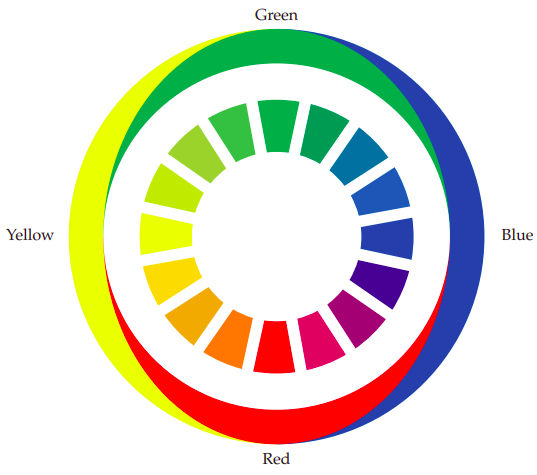
\includegraphics[width=0.9\textwidth]{HSB}
        \caption{Hering's idea of opponent colors \cite{SPCbook}}
\label{HSB}
\end{figure}

\section{Hue cancellation}
In 1957 two American psychologists by 
the names of Dorothea Jameson and Leo Hurvich 
set about developing a new way of quantifying 
Herings’ theory regarding colour-opponency, 
dubbed ‘Hue cancellation’. Jameson and Hurvich 
reasoned that given a light that appears to be of a 
certain colour, one could cancel the colour, or one of 
its specific colour components by adding a certain 
amount of its opponent colour. \cite{SPCbook} 
The two psychologists provided the important 
quantitative data needed to revive Herring’s 
colour-opponent theory by conducting hue 
cancellation experiments for lights across the spectrum. \cite{SPCbook}\\
Jameson and Hurvich conducted their experiments 
by presenting a participant, the observer, with a 
monochromatic test light. If the test light was judged 
to be red in appearance, the participant would be asked 
to cancel out precisely the red component by 
adding a certain amount of its opponent colour green. 
If the test light was judged to be green in appearance, 
the participant would be asked to cancel 
out the green using a red light.\\
\begin{figure}[h!]
        \centering
        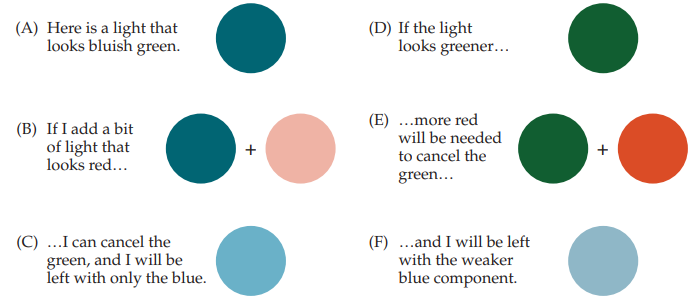
\includegraphics[width=0.9\textwidth]{hue}
        \caption{A hue cancellation experiment involving green colour components \cite{SPCbook}}
\label{hue}
\end{figure}

\section{Color in the visual cortex}
The famous studies of V1 and V2 cortex 
in monkeys by Livingstone and Hubel, 1984,
supported the modular concept and linked it 
to parallel processing in the retina and 
the lateral geniculate nucleus (LGN). 
The landmark studies of De Valois (1965) 
first suggested that color opponent neurons 
existed in the primate visual system and 
could be important for color vision. \cite{shapley2011color}
The opponent cells found in the brain 
are of two types, single opponent cells
and double opponent cells.\\
And of single opponent cells there are
two kinds. First, the L–M or M–L cells that 
receive input from long wavelength (L) cones 
opposed by signals from middle wavelength(M) cones, 
for simplicity called red/green opponent cells.
The S/(L + M) opponent cells are sometimes 
referred to as blue/yellow opponent cells. \cite{shapley2011color}
In figure \ref{opp_cells} (a) and (b) we can see
an example of a single opponent cell that is excited 
by wavelengths corresponding to the red 
color in its center and inhibited by the green color 
in its outer layer. From the figure can be seen that single
opponent cells convey information about color in
a broad area. \cite{SPCbook}\\
The defining characteristic of a double-opponent 
cell is that it is strongly responsive to 
color patterns but weakly or non-responsive
to full-field color stimuli. \cite{shapley2011color}
The double-opponent cells were described as strongly 
responsive to color bars but 
insensitive to full-field color stimuli.\cite{shapley2011color}
Thus being able to detect chromatic edges. \cite{SPCbook}
The center of of each double opponent cell gets excitatory 
input from one cone type and inhibitory from another. 
The pattern is opposite in the outer layer.
In figure \ref{opp_cells} (c) (d) the behavior of 
the double opponent cell can be seen. Notice the difference
of excitatory input near the edge.\\
Studies in which parts of the brain are 
connected to color come from cases of achromatopsia.
Which is a condition that results in loss of 
color vision after brain damage. Vision is largely 
intact but color perception is impaired. \cite{SPCbook}
\begin{figure}[h!]
        \centering
        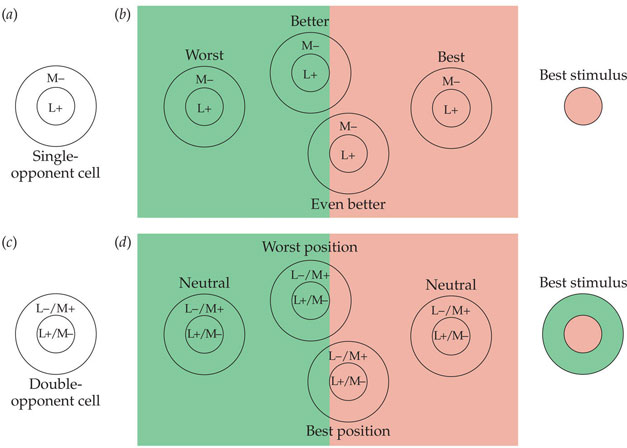
\includegraphics[width=0.9\textwidth]{opp_cells}
        \caption{Color opponent receptive fields \cite{SPCbook}}
\label{opp_cells}
\end{figure}

\section{Adaption and Afterimages}
The principle of dark adaption \cite{lightanddark} 
can be extended to colour. That is, adaption can 
be colour specific, as seen in the phenomena known as 
negative afterimages. A negative afterimage is, as the 
name suggests, an afterimage seen after viewing a stimulus 
composed of one or more colour components and then subsequently 
viewing an achromatic region. The achromatic region will appear 
to take on the opponent colour/colours of the initial stimulus, 
known as the adapting stimulus. Figure \ref{afterimages} illustrates two varying 
examples of adapting stimuli (B) (C), and the achromatic regions 
(A) (D) that combined result in negative afterimages.\\
After staring at the black dot in figure \ref{afterimages}B, and then immediately 
exposing one’s gaze to the black dot in figure \ref{afterimages}A, the achromatic 
circles surrounding it will appear to take on the opponent-colours 
of the circles seen in figure \ref{afterimages}B. 
By staring at the adapting stimuli (B), 
one’s retina is being exposed to several coloured dots, one of 
these being red. The red-sensing cone cells, or L-cones, will 
be stimulated to a much higher degree than the M or S cones, which 
results in one seeing the colour red. After diverting one’s gaze 
to the achromatic image (A), the opponent process is stimulated, 
due to the red-sensing cones being more adapted than the M or S cones. \cite{SPCbook} 
This adaption results in the red-green opponent colour mechanism 
overshooting the point at which the mechanism is not generating 
any form of signal, and “landing” on the green side. \cite{SPCbook} As a 
result of this, the topmost grey circle (A) will take on a 
green appearance until the opponent colour mechanism moves 
back to the point where it no longer is generating a signal.\\
\begin{figure}[h!]
        \centering
        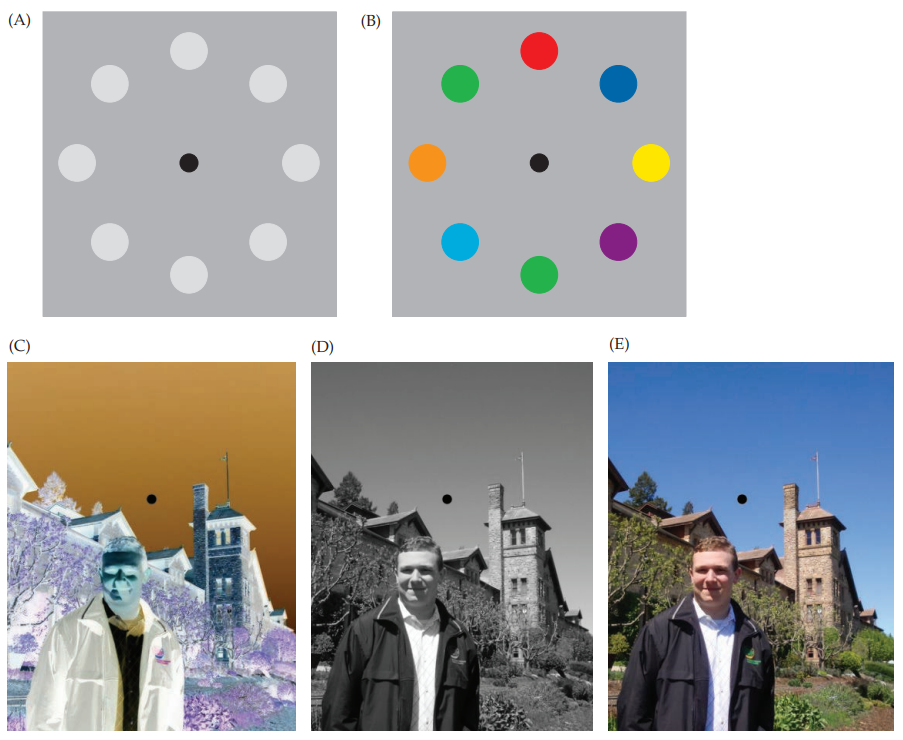
\includegraphics[width=0.9\textwidth]{afterimages}
        \caption{Two examples of negative afterimages \cite{SPCbook}}
\label{afterimages}
\end{figure}

\cleardoublepage
\bibliographystyle{unsrt}
\bibliography{main}

\end{document}